\documentclass{article}

\usepackage[english]{babel}
\usepackage[utf8]{inputenc}
\usepackage{graphicx}
\usepackage{hyperref}
\usepackage{placeins}
\usepackage{csquotes}
\usepackage{tikz}
\usetikzlibrary{positioning}

%\usepackage[left=1.5cm,right=1.5cm,top=2cm,bottom=2cm]{geometry}
\title{LSINF2345 - Course project \\ A Simulated Bike Race}
\author{Alexandre Hauet \and Florian Thuin}
\date{\today}

\def\blurb{\textsc{Université catholique de Louvain\\
  École polytechnique de Louvain\\
  Pôle d'ingénierie informatique}}
\def\clap#1{\hbox to 0pt{\hss #1\hss}}%
\def\ligne#1{%
  \hbox to \hsize{%
    \vbox{\centering #1}}}%
\def\haut#1#2#3{%
  \hbox to \hsize{%
    \rlap{\vtop{\raggedright #1}}%
    \hss
    \clap{\vbox{\vfill\centering #2\vfill}}%
    \hss
    \llap{\vtop{\raggedleft #3}}}}%


\begin{document}

\begin{titlepage}
\thispagestyle{empty}\vbox to 1\vsize{%
  \vss
  \vbox to 1\vsize{%
    \haut{\raisebox{-5mm}{\includegraphics[width=2.5cm]{logo_ucl.pdf}}}{\blurb}{\raisebox{-5mm}{\includegraphics[scale=0.20]{ingi_logo.png}}}
    \vfill
    \ligne{\Huge \textbf{\textsc{LSINF2345}}}
     \vspace{5mm}
    \ligne{\huge \textbf{\textsc{Course project }}}
     \vspace{15mm}
    \ligne{\Large \textbf{\textsc{A Simulated Bike Race}}}
    \vspace{5mm}
    \ligne{\large{\textsc{\today}}}
    \vfill
    \vspace{5mm}
    \ligne{%
         \textsc{Group 10\\Alexandre Hauet\\Florian Thuin}
      }
      \vspace{5mm}
    }%
  \vss
  }
\end{titlepage}

\begin{abstract}
    This report describes the results and solutions to the three problems
    linked to the \textbf{bike race} project, using Erlang and Riak along with
    a key-value store (a distributed hash table). Information on compilation and
    execution can be found in the attached \verb#README.md#, a flavored-markdown
    Readme in GitHub style.
\end{abstract}

\section*{Problem 0}
For the first problem of the project, we needed to start by setting the track,
where no biker fails and no special consideration has been given to broadcasting
messages. We use the best-effort broadcast (beb) to implement this problem.
\newline

At the beginning of the race, each biker starts with an unique \verb#Pid# given by the
user at start using \verb#biker:start_race(Pid, NbrOfPlayers)#. To implement the
best-effort broadcast, we took advantage of riak and the given key-value store
(kvstore\footnote{\url{https://github.com/rumapaul/kvstore}}). The race works
as a sequence of rounds limited by time, during which each node will store its
decision in the key-value store. Using the unique id of the biker as its key allow
each biker to retrieve the decision of other bikers. As there are no loops in
Erlang, the BEB is implemented as a tail-recursive function named \verb#beb_loop#
in the module \verb#beb#.\newline

According to the course the best-effort broadcast properties are :
\begin{description}
    \item[Best-effort-Validity] : If $p_{i}$ and  $p_{j}$ are correct, then
    any broadcast by $p_{i}$ is eventually delivered by $p_{j}$
    \item[No duplication] : No message delivered more than once
    \item[No creation] : No message delivered unless broadcast
\end{description}

Here is how our algorithm fulfill the properties :
\begin{itemize}
\item We use a key-value store to share information (decision) between the
bikers. So when a biker ($b_{i}$) stores its decision in it, it will eventually
be written and then be readable by every other bikers (it is a property of the
kvstore);
\item The message are not duplicated, they are stored only at one key in the
key-value store by the bikers;
\item No messages are created without an input (whether from the user himself,
whether from the default decision after a timeout).
\end{itemize}

The results given by our algorithm effectively matches the properties of a
best-effort broadcast algorithm.\newline

We can observe strange behavior. Each node has its own way to manage the
conflict between \enquote{behind} (or \enquote{follow}) decisions. If we have a
cycle (for example the biker $A$ follows the biker $B$, the biker $B$ follows the
biker $C$ and the biker $C$ follows the biker $A$), the view of the race will not be
the same for each node anymore.

\begin{figure}[!ht]
    \begin{center}
        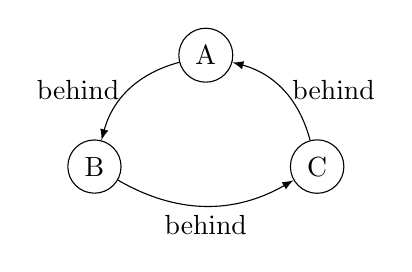
\begin{tikzpicture}[auto, on grid, node distance=2cm]
            \node[draw, circle] (A) {A};
            \node[draw, circle, below left of = A] (B) {B};
            \node[draw, circle, below right of = A] (C) {C};

            \path[-latex] (A) edge [bend right] node [left] {behind} (B);
            \path[-latex] (B) edge [bend right] node [below] {behind} (C);
            \path[-latex] (C) edge [bend right] node [right] {behind} (A);
        \end{tikzpicture}
        \caption{Conflict situation}

        \bigskip
        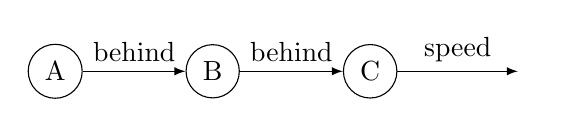
\begin{tikzpicture}[auto, on grid, node distance=2cm]
            \node[draw, circle] (A) {A};
            \node[draw, circle, right of = A] (B) {B};
            \node[draw, circle, right of = B] (C) {C};
            \node[right of = C] (D) {};

            \path[-latex] (A) edge node {behind} (B);
            \path[-latex] (B) edge node {behind} (C);
            \path[-latex] (C) edge node {speed} (D);
        \end{tikzpicture}
        \caption{How $A$ can solve it}

        \bigskip
        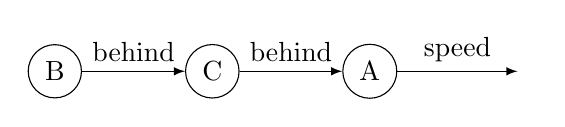
\begin{tikzpicture}[auto, on grid, node distance=2cm]
            \node[draw, circle] (B) {B};
            \node[draw, circle, right of = B] (C) {C};
            \node[draw, circle, right of = C] (A) {A};
            \node[right of = A] (D) {};

            \path[-latex] (A) edge node {speed} (D);
            \path[-latex] (B) edge node {behind} (C);
            \path[-latex] (C) edge node {behind} (A);
        \end{tikzpicture}
        \caption{How $B$ can solve it}
    \end{center}
\end{figure}
\FloatBarrier

We can see that, based on how nodes are involved in a conflict, they can
decide to change the decision of another node (by setting its decision to its
previous speed choice) as if they were the leader and that leads to divergences
between the knowledge of the race of each node. That's what problem 1 will solve.

\section*{Problem 1}

For this problem, we need to guarantee the same view for all bikers. As we saw
in the problem 0, bikers can have different views because they read their decision
first and then the one of the other bikers. To solve this problem, we need to
implement a total-order broadcast. One of the major
differences between best-effort broadcast and total order broadcast is that in
the latter, the processes must deliver and execute all decisions according to
the same order. \newline

The solution to apply this, keeping the logic of the algorithm for problem 0, is
to set an order in the reading of the values such that there is a leader from
which we read the view of the race and everyone applies it. It can be done by
looping on the key-value store exactly in the same way in each node once every
decision is in it, and applying the exact same conflict resolution technique
for each node. That's what our algorithm does with the tail-recursive function
\verb#tob_loop# in the module \verb#tob#. If you want to switch from \verb#beb#
to \verb#tob#, you can just comment out one line in \verb#start_race/2# of module
\verb#biker#.

\begin{figure}[!ht]
    \begin{center}
        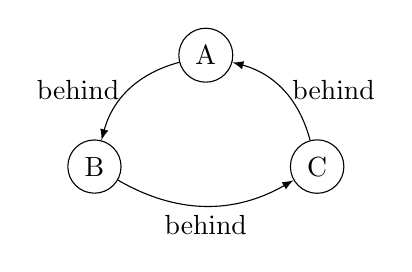
\begin{tikzpicture}[auto, on grid, node distance=2cm]
            \node[draw, circle] (A) {A};
            \node[draw, circle, below left of = A] (B) {B};
            \node[draw, circle, below right of = A] (C) {C};

            \path[-latex] (A) edge [bend right] node [left] {behind} (B);
            \path[-latex] (B) edge [bend right] node [below] {behind} (C);
            \path[-latex] (C) edge [bend right] node [right] {behind} (A);
        \end{tikzpicture}
        \caption{Conflict situation}

        \bigskip
        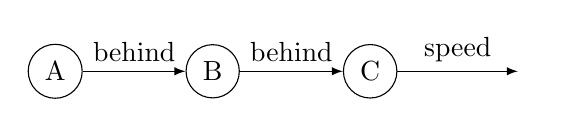
\begin{tikzpicture}[auto, on grid, node distance=2cm]
            \node[draw, circle] (A) {A};
            \node[draw, circle, right of = A] (B) {B};
            \node[draw, circle, right of = B] (C) {C};
            \node[right of = C] (D) {};

            \path[-latex] (A) edge node {behind} (B);
            \path[-latex] (B) edge node {behind} (C);
            \path[-latex] (C) edge node {speed} (D);
        \end{tikzpicture}
        \caption{How $A$ will solve it}

        \bigskip
        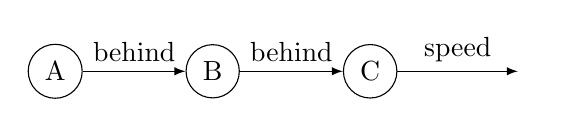
\begin{tikzpicture}[auto, on grid, node distance=2cm]
            \node[draw, circle] (B) {A};
            \node[draw, circle, right of = B] (C) {B};
            \node[draw, circle, right of = C] (A) {C};
            \node[right of = A] (D) {};

            \path[-latex] (A) edge node {speed} (D);
            \path[-latex] (B) edge node {behind} (C);
            \path[-latex] (C) edge node {behind} (A);
        \end{tikzpicture}
        \caption{How $B$ will solve it}
    \end{center}
\end{figure}
\FloatBarrier

The result is such that everyone has the same information and it results
as giving the same view.

\section*{Problem 2}

As we were short in time, we couldn't implement this problem. But here is
how it could have been done:

\begin{itemize}
    \item There is a \verb#ping()# function that can be called such that you can
    see if a node is alive (if it is, it will answer pong and a value);
    \item As we can suppose a perfect point-to-point link (nodes are on the
    same machine) and a very short time of delivery (because messages are sent
    and receive on local host), if we don't have answer to our \verb#ping()# in
    a second, we can assume the node has crashed and the detection is perfect;
    \item If the node is crashed, we don't have to read from its key anymore,
    we can assume each decision he takes will be of kind \verb#{speed, 0}#
    (which means: no move, realistic if he falls down). We maintain a list
    of crashed node such that we never read again from them and we don't run
    the perfect failure detector on them anymore (because of crash-stop);
    \item We repeated the above step as long as the race is running.
\end{itemize}

\section*{Conclusion}

There was a steep learning curve to get started with this project. It took time
to start coding, but we learned a lot from the power of Erlang and the power
of Riak. We hope we showed it and our motivation to give our best to solve this
project.

\end{document}
